\chapter{Waves, Phase, and Complex Amplitude: The Minimal Language of Interference}
\label{chap:e01}

\begin{chapteropening}
Imagine you are standing behind the focus of a telescope, and a beam of starlight has just fallen in. What is it, physically? It is a stretch of electric field swinging rapidly back and forth: how rapidly? One round trip takes only a few femtoseconds, trillions of times faster than a single blink of your eye. Yet when this light finally becomes data, that rapid swinging has ``vanished,'' and the detector leaves behind only a quiet number: the intensity, or the photon count. Where did the swinging go? Where did the phase go?

What this chapter sets out to do is to build up the ``language of the wave'' from the ground up: first we write down a stretch of monochromatic electromagnetic wave; then we learn to use a ``rotating arrow'' (the complex amplitude) to hold both its amplitude and its phase at once; then we work out why the detector can see only the square of the amplitude and not the phase itself; and finally we let two beams of light meet and watch how interference turns the ``invisible phase difference'' back into ``visible brightness and darkness.'' These few things are the shared alphabet of all the later chapters on coherence, interference, and intensity correlation.
\end{chapteropening}

\section{The Monochromatic Electromagnetic Wave: A Stretch of Rapidly Swinging Electric Field}
\label{sec:e01-wave}

Let us first set the picture. Within a sufficiently narrow frequency channel, starlight can be approximated as a train of \textbf{monochromatic light}: it has a single frequency, like a pure tone. What is really oscillating is the electric field strength at some point in space: it goes up and down with time, like a string that swings steadily after being plucked. Mathematically we write it as

\begin{equation}
  E(t)=E_0\cos(\omega t+\phi),\qquad \omega=2\pi\nu .
  \label{eq:e01-monochromatic}
\end{equation}
\begin{formulaexplain}
\(E(t)\) is the electric field at time \(t\); \(E_0\) is the amplitude (the maximum extent of the swing); \(\omega\) is the angular frequency, \(\nu\) is the ordinary frequency, and the two differ by a factor of \(2\pi\); \(\phi\) is the initial phase, which sets where the swing is at \(t=0\).
\end{formulaexplain}

Let us pin down each symbol. \(E(t)\) is the electric field; in CGS units its dimension is \({\rm statvolt\,cm^{-1}}\), but for the derivations of this chapter its actual magnitude does not matter: what matters is \emph{how it varies with time}. \(E_0\) is the maximum height of this swing, that is, the amplitude, which likewise carries the dimension of electric field. \(\phi\) is the initial phase, in units of radians; it is a pure angle and dimensionless, and you can read it as ``at the instant \(t=0\), how far into the cycle the swing has progressed.''

The quantity \(\omega t+\phi\) inside the parentheses is called the \textbf{instantaneous phase}: as time passes, \(\omega t\) increases uniformly, and the cosine swings again and again from \(+1\) down to \(-1\) and back. The unit of the angular frequency \(\omega\) is \({\rm rad\,s^{-1}}\); it tells us how fast the phase advances. Its relation to the ordinary frequency \(\nu\) (in Hz, that is, how many full cycles per second) is \(\omega=2\pi\nu\), because one full turn is \(2\pi\) radians. The period is \(T=1/\nu=2\pi/\omega\).

Now let us put in real numbers to feel how fast this is. Visible light has a frequency of about

\[
  \nu\simeq 4\times10^{14}\ {\rm Hz}\ (\text{red light})\quad\text{to}\quad 8\times10^{14}\ {\rm Hz}\ (\text{blue light}),
\]

so one period is only

\[
  T=\frac{1}{\nu}\simeq\frac{1}{5\times10^{14}\ {\rm Hz}}=2\times10^{-15}\ {\rm s}=2\ {\rm fs}.
\]

That is, the electric field of visible light completes one full up-and-down swing every two femtoseconds. What kind of a scale is a femtosecond (\(10^{-15}\) second)? In one femtosecond, light travels only \(0.3\ \mu{\rm m}\), less than a hundredth of the diameter of a human hair. Any conventional astronomical detector, whether a CCD pixel, a photomultiplier tube, or an avalanche photodiode, has a response time of at least the nanosecond (\(10^{-9}\) second) scale, \(10^{5}\)--\(10^{6}\) times slower than one optical period (comparing ``at least \(1\ {\rm ns}\)'' with ``about \(2\ {\rm fs}\)'' gives \(1\ {\rm ns}/2\ {\rm fs}\approx5\times10^{5}\); for a CCD with integration times down to the microsecond scale it is slower still).

This brings out a key fact that runs through the whole book: the detector is ``too slow'': it simply cannot keep up with the field's cycle-by-cycle positive and negative swings. In the time it takes the detector to blink its ``electronic eye'' once, the field has already swung up and down hundreds of thousands or even millions of times. It cannot record each swing; it can only \emph{smooth} these rapid oscillations over its own response time, leaving behind an average energy. So the rapidly varying part of \(E(t)\), the part carrying the phase information, is \textbf{directly invisible} to the detector. We will see later that it is precisely this that forces people to invent interferometry and correlation measurements: the only way to turn the ``invisible phase'' back into ``visible intensity.''

\section{Complex Amplitude: Packing Amplitude and Phase into One Rotating Arrow}
\label{sec:e01-phasor}

Equation~\eqref{eq:e01-monochromatic} is a bit clumsy: every time we discuss adding two beams together and how the phase difference changes, we have to fiddle with a pile of product-to-sum cosine formulas. Is there a cleverer notation that packs the two things, \emph{amplitude} and \emph{phase}, in one stroke, and also makes addition simple? Yes: this is the \textbf{complex amplitude} (also called a phasor).

First the picture. Think of the cosine as the projection onto the horizontal axis of an arrow that starts at the origin and rotates uniformly about it: the \emph{length} of the arrow is the amplitude \(E_0\), and the \emph{angle} the arrow points to is the instantaneous phase \(\omega t+\phi\). The arrow turns counterclockwise at angular velocity \(\omega\)\footnote{Here we have chosen the \(e^{+i\omega t}\) time convention: the arrow rotates counterclockwise, and positive frequencies take \(+i\omega t\). Within this chapter it is entirely self-consistent, and none of the conclusions are affected. One reminder, to avoid confusion when interfacing later: when we introduce the positive/negative-frequency field operators \(\hat E^{(+)},\hat E^{(-)}\) for second quantization, the positive-frequency part \(\hat E^{(+)}\) containing the annihilation operator \(\hat a\) usually evolves as \(e^{-i\omega t}\), so the arrow turns the opposite way from here. The two conventions are just mirror-image notations for the same physics: replacing every \(i\) here with \(-i\) (equivalent to viewing the arrow as turning clockwise) interfaces smoothly, with the physical content unchanged.}, and its shadow on the real axis (the horizontal direction) is exactly \(E_0\cos(\omega t+\phi)\). So ``a stretch of oscillating field'' is translated into ``a rotating arrow.'' Since we want to describe an arrow in the plane, complex numbers are the most natural choice: a point in the complex plane inherently carries the two pieces of information ``length'' and ``angle.''

We package the arrow's appearance at \(t=0\) (length \(E_0\), angle \(\phi\)) into a complex number:

\begin{equation}
  \mathcal{E}=E_0e^{i\phi},\qquad E(t)=\operatorname{Re}\!\left[\mathcal{E}\,e^{i\omega t}\right].
  \label{eq:e01-phasor}
\end{equation}
\begin{formulaexplain}
\(\mathcal E\) is the complex amplitude; its modulus \(|\mathcal E|=E_0\) is the amplitude, and its argument \(\arg\mathcal E=\phi\) is the phase. Multiplying by the rotation factor \(e^{i\omega t}\) sets the arrow turning, and taking the real part \(\operatorname{Re}\) (the horizontal shadow) recovers the real electric field \(E(t)\).
\end{formulaexplain}

Let us verify that this notation really recovers Eq.~\eqref{eq:e01-monochromatic}. Using Euler's formula \(e^{i\theta}=\cos\theta+i\sin\theta\) (this is the definition of the complex exponential, which the book will use again and again), we expand step by step:

\[
  \mathcal{E}\,e^{i\omega t}
  =E_0e^{i\phi}\,e^{i\omega t}
  =E_0\,e^{i(\omega t+\phi)}
  =E_0\bigl[\cos(\omega t+\phi)+i\sin(\omega t+\phi)\bigr].
\]

Taking the real part (discarding the imaginary part carrying \(i\)):

\[
  \operatorname{Re}\!\left[\mathcal{E}\,e^{i\omega t}\right]
  =E_0\cos(\omega t+\phi)=E(t).
\]

Not a step off: exactly the original field. So no information is lost in the complex amplitude \(\mathcal E\): \(|\mathcal E|=|E_0e^{i\phi}|=E_0\) gives the amplitude, and \(\arg\mathcal E=\phi\) gives the phase. \(\mathcal E\) carries the same dimension as the electric field, while the \(e^{i\phi}\) part is a dimensionless pure direction.

The advantage of this notation only truly shows itself in the next section, when two beams are added: adding cosines is troublesome, but adding complex numbers is just vector addition of arrows placed head to tail, much simpler. This is why, from now on, we almost always do our bookkeeping first in the world of complex amplitudes, and only take the real part or the modulus at the end to fall back into the real world.

\section{Intensity: Why the Detector Sees Only the Square of the Amplitude}
\label{sec:e01-intensity}

Back to the core question: the detector cannot see the rapid swinging, so what exactly does it record? The answer is the \textbf{intensity}, that is, the average of the square of the field over the response time. Physically, the detector absorbs the energy of the light, and the energy density carried by the electromagnetic field is proportional to the square of the field. So the quantity left behind by the detector is proportional to \(\langle E^2(t)\rangle\), where the angle brackets denote ``a time average over the detector's response time.''

Let us compute this average step by step, skipping nothing. Starting from \(E(t)=E_0\cos(\omega t+\phi)\):

\[
  E^2(t)=E_0^2\cos^2(\omega t+\phi).
\]

The key step is to use the double-angle identity for the cosine, \(\cos^2\theta=\tfrac12\bigl[1+\cos(2\theta)\bigr]\) (a standard trigonometric identity, obtainable by solving \(\cos 2\theta=2\cos^2\theta-1\)), to split the square open:

\[
  E^2(t)=E_0^2\cdot\frac{1+\cos\!\bigl(2\omega t+2\phi\bigr)}{2}
  =\frac{E_0^2}{2}+\frac{E_0^2}{2}\cos\!\bigl(2\omega t+2\phi\bigr).
\]

Now take the time average. The first term on the right, \(E_0^2/2\), is a constant, and its average is itself. The second term is a cosine oscillating rapidly at \(2\omega\) (twice the optical frequency, an even shorter period): over the detector's long response time it swings up and down through countless full periods, the positive parts and the negative parts cancelling exactly, so its average is zero. This is precisely the ``smoothing'' spoken of in the previous section:

\[
  \bigl\langle\cos(2\omega t+2\phi)\bigr\rangle_{\rm det}\approx 0
  \quad\Longrightarrow\quad
  \bigl\langle E^2(t)\bigr\rangle_{\rm det}=\frac{E_0^2}{2}.
\]

So the intensity left behind by the detector is proportional to

\begin{equation}
  I\ \propto\ \bigl\langle E^2(t)\bigr\rangle_{\rm det}=\frac{E_0^2}{2}=\frac{1}{2}\,|\mathcal E|^2 .
  \label{eq:e01-intensity}
\end{equation}
\begin{formulaexplain}
\(I\) is the detected intensity; \(\langle\cdots\rangle_{\rm det}\) is the time average over the detector's response time; that \(1/2\) is precisely the result of averaging \(\cos^2\) over one period; \(|\mathcal E|^2\) is the modulus squared of the complex amplitude. The phase \(\phi\) has \emph{vanished} from the final result.
\end{formulaexplain}

Please stare especially hard at what disappears at the end of this equation: \(\phi\) is gone. The intensity depends only on the amplitude \(E_0\) (or \(|\mathcal E|\)), and not at all on the phase. From the complex-amplitude viewpoint this is even more transparent: \(|\mathcal E|^2=|E_0e^{i\phi}|^2=E_0^2\), the modulus of that \(e^{i\phi}\) is 1, and taking the modulus squared swallows the phase factor entirely. No matter which direction the rotating arrow initially points, as long as its length is the same, the measured intensity is the same.

Physically this sentence is a cornerstone of the whole book: \textbf{the phase of a single beam of light is not directly recorded by the detector}. It is like a hidden degree of freedom; the intensity data in your hands know nothing about it. But earlier chapters said the phase is important. Isn't this a contradiction? It is not: the absolute phase of a single beam really cannot be measured, but the \emph{phase difference} of two beams can, because the phase difference changes the length of the resultant arrow, and thereby changes the intensity. This is exactly where interference comes into play, and we go to see it right away.

(A notational convention: that constant \(1/2\), along with various geometrical and efficiency factors, is often absorbed into the proportionality constant in later text and written as \(I\propto|\mathcal E|^2\). This chapter writes the \(1/2\) out explicitly to make the step of ``smoothing away the rapid oscillation'' plain to see.)

\section{When Two Beams Meet: How Interference Turns a Phase Difference Back into Brightness and Darkness}
\label{sec:e01-interference}

Now let two beams of monochromatic light (say, from the same star, having taken two different paths) fall on the same detector. The crucial physical order is: \textbf{the fields are added first, and the intensity is squared afterward}. This order cannot be reversed. Because the electromagnetic field obeys the superposition principle, the fields of the two beams at the same point add as vectors; and what the detector measures is the energy of that resultant field \emph{after} the addition. Doing this with complex amplitudes is the least laborious: two arrows head to tail, mere vector addition.

Let the complex amplitudes of the two beams be \(\mathcal E_1\) and \(\mathcal E_2\); the complex amplitude of the resultant field is then \(\mathcal E_1+\mathcal E_2\). The intensity is proportional to its modulus squared:

\begin{equation}
  I\ \propto\ |\mathcal E_1+\mathcal E_2|^2
  =|\mathcal E_1|^2+|\mathcal E_2|^2+2\,\operatorname{Re}\!\bigl(\mathcal E_1\mathcal E_2^{\ast}\bigr).
  \label{eq:e01-interference}
\end{equation}
\begin{formulaexplain}
\(\mathcal E_1,\mathcal E_2\) are the complex amplitudes of the two beams; the first two terms \(|\mathcal E_1|^2,|\mathcal E_2|^2\) are their separate intensities; the third term \(2\operatorname{Re}(\mathcal E_1\mathcal E_2^{\ast})\) is the \emph{interference term}, where the star \({}^\ast\) denotes complex conjugation. It is this term that makes the total intensity larger or smaller.
\end{formulaexplain}

Let us derive this expansion honestly. For any complex number \(z\), the modulus squared is it times its own conjugate: \(|z|^2=z\,z^{\ast}\). Let \(z=\mathcal E_1+\mathcal E_2\); its conjugate is \(\mathcal E_1^{\ast}+\mathcal E_2^{\ast}\), and multiplying term by term:

\[
  |\mathcal E_1+\mathcal E_2|^2
  =(\mathcal E_1+\mathcal E_2)(\mathcal E_1^{\ast}+\mathcal E_2^{\ast})
  =\mathcal E_1\mathcal E_1^{\ast}+\mathcal E_2\mathcal E_2^{\ast}
  +\mathcal E_1\mathcal E_2^{\ast}+\mathcal E_2\mathcal E_1^{\ast}.
\]

The first two terms are \(|\mathcal E_1|^2\) and \(|\mathcal E_2|^2\). The last two terms, \(\mathcal E_1\mathcal E_2^{\ast}\) and \(\mathcal E_2\mathcal E_1^{\ast}\), are conjugates of each other, and since ``a complex number plus its conjugate equals twice its real part'' (\(z+z^{\ast}=2\operatorname{Re}z\)), together they are precisely \(2\operatorname{Re}(\mathcal E_1\mathcal E_2^{\ast})\). This gives Eq.~\eqref{eq:e01-interference}.

Next, let us substitute the explicit form of the complex amplitude to make the phase appear. Writing \(\mathcal E_1=E_1e^{i\phi_1}\) and \(\mathcal E_2=E_2e^{i\phi_2}\), first compute the product:

\[
  \mathcal E_1\mathcal E_2^{\ast}
  =E_1e^{i\phi_1}\cdot E_2e^{-i\phi_2}
  =E_1E_2\,e^{i(\phi_1-\phi_2)}
  =E_1E_2\bigl[\cos(\phi_1-\phi_2)+i\sin(\phi_1-\phi_2)\bigr].
\]

Taking the real part and discarding the imaginary part, the interference term becomes

\[
  2\,\operatorname{Re}\!\bigl(\mathcal E_1\mathcal E_2^{\ast}\bigr)
  =2E_1E_2\cos(\phi_1-\phi_2).
\]

So the total intensity of the two beams is written as

\[
  I\ \propto\ E_1^2+E_2^2+2E_1E_2\cos(\phi_1-\phi_2).
\]

Look at the last term of this equation: it depends only on the \textbf{phase difference} \(\Delta\phi=\phi_1-\phi_2\), not on the individual absolute phases. This is exactly what echoes the conclusion of the previous section: the absolute phase cannot be measured, but the phase difference can be made manifest through the intensity. Read it in three cases:

\begin{itemize}
  \item \textbf{Constructive interference}: \(\Delta\phi=0\) (or an integer multiple of \(2\pi\)), \(\cos\Delta\phi=+1\), and the interference term takes its maximum positive value. The two arrows superpose in the same direction, the resultant arrow is longest, and the intensity surges to the peak \(E_1^2+E_2^2+2E_1E_2=(E_1+E_2)^2\). If \(E_1=E_2=E_0\), the peak is \(4E_0^2\), \emph{four} times the single-beam intensity \(E_0^2\), not twice. The extra energy is precisely the result of interference ``redistributing'' it.
  \item \textbf{Destructive interference}: \(\Delta\phi=\pi\), \(\cos\Delta\phi=-1\), and the interference term takes its maximum negative value. The two arrows point in opposite directions, the resultant arrow is shortest, and the intensity drops to the trough \((E_1-E_2)^2\). For equal intensities \(E_1=E_2\), it is \emph{completely dark} here.
  \item \textbf{Averaged away}: if the phase difference \(\Delta\phi\) is unstable, varying rapidly and irregularly over the measurement time (the two beams cannot ``remember'' each other's phase), then \(\cos\Delta\phi\) is now positive, now negative, averaging toward zero, the interference term vanishes, and only \(I\propto E_1^2+E_2^2\) remains: the two beams add simply, like incoherent street lamps. This question of ``whether the phase difference stays stable'' is precisely \textbf{coherence}, which is the protagonist of the whole book from Chapter~\ref{chap:e05} onward.
\end{itemize}

To close this section in one sentence: interference is a ``phase-difference translation machine'': it translates the phase difference \(\Delta\phi\), which the detector cannot see, into visible brightness and darkness (the highs and lows of the intensity). All the various interference and correlation measurements discussed in this book are, at heart, reading out this \(\cos\Delta\phi\) with different tricks.

\begin{figure}[tbp]
\centering
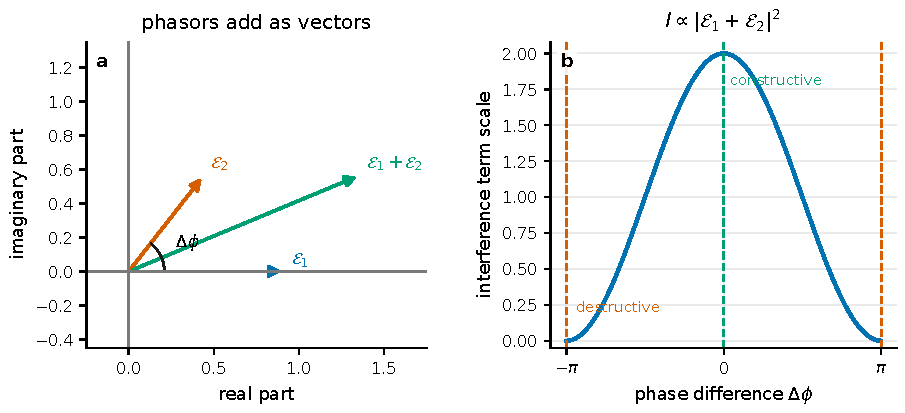
\includegraphics[width=0.85\linewidth]{figures/generated/chapter_01/ch01_phase_interference.pdf}
\caption{The basic picture of complex amplitudes and the interference of two beams. The complex amplitude is an arrow whose length is the amplitude and whose direction is the phase; the two beams first undergo vector addition of the arrows, and the detector then takes the square of the length of the resultant arrow. The phase difference \(\Delta\phi\) determines whether the interference term reinforces (constructive), cancels (destructive), or is averaged away when the phase varies wildly.}
\label{fig:e01-phase-interference}
\end{figure}

\section{Geometric Phase: Where the Path Difference Comes From}
\label{sec:e01-geometry}

The phase difference \(\Delta\phi\) of the previous section is still rather abstract. In astronomical observation, its most common source is in fact very concrete and very geometric: \textbf{the two beams travel paths of unequal length}. This section turns this ``path difference'' step by step into a phase difference.

First set the picture. Let there be a very distant star; when the light it emits reaches the ground, the wavefront (the surface of equal phase) is almost a large flat sheet, advancing along the source direction \(\bm s\) (a unit vector pointing to the star). On the ground there are two telescopes, whose positions differ by a \textbf{baseline vector} \(\bm B\), the vector pointing from the first to the second, in units of centimetres. Because the two telescopes are not on the same wavefront perpendicular to \(\bm s\), one and the same wavefront reaches one of them first and must travel a little extra to reach the other. This ``little extra'' is the path difference.

How long is the extra path? Just project the baseline \(\bm B\) onto the source direction \(\bm s\). The length of the projection of a vector onto a given direction is precisely the dot product, so the path difference is

\[
  \Delta \ell=\bm B\cdot\bm s .
\]

The geometric meaning of this step must be seen clearly: \(\bm B\cdot\bm s=|\bm B|\cos\theta\), where \(\theta\) is the angle between the baseline and the source direction. If the star lies straight ahead of the baseline (\(\bm B\) parallel to \(\bm s\)), the projection is longest and the path difference greatest; if the star lies straight above the baseline (\(\bm B\perp\bm s\)), the projection is zero, the two telescopes have equal paths to the same wavefront, and there is no path difference. This agrees with everyday experience: only for light arriving at a slant is there a lead-and-lag between the two receiving points.

Now let us convert ``the extra stretch of path'' into ``the extra amount of phase turned.'' Here we need a fact that has not yet been formally stated, but that can be derived from the picture of Section~\ref{sec:e01-wave} right away: as the wave advances by one \textbf{wavelength} \(\lambda\) in space, the phase advances by exactly \(2\pi\) (one full turn). Why? Return to the time picture set up in Section~\ref{sec:e01-wave}: each time the field passes one period \(T\), the instantaneous phase increases by \(\omega T=2\pi\) (this is precisely the definition of ``one full turn per period''). And in that same time \(T\), a wave propagating at the speed of light \(c\) advances exactly a distance

\[
  \lambda\ \equiv\ cT=\frac{c}{\nu}=\frac{2\pi c}{\omega}.
\]

The spatial length corresponding to this ``phase accumulating exactly one full turn of \(2\pi\)'' is the wavelength. So ``one period has passed in time'' and ``one wavelength has been advanced in space'' are two ways of saying the same thing, with the phase advancing by exactly \(2\pi\) in both. In this way, \(\lambda\) is not a new symbol appearing out of nowhere: it is directly determined from the \(\nu\) (or \(\omega\)) honed repeatedly in Section~\ref{sec:e01-wave} through \(\lambda=c/\nu\). Substituting the visible-light frequency \(\nu\simeq5\times10^{14}\ {\rm Hz}\) from there, we get \(\lambda=c/\nu\approx(3\times10^{10}\ {\rm cm\,s^{-1}})/(5\times10^{14}\ {\rm Hz})=6\times10^{-5}\ {\rm cm}=0.6\ \mu{\rm m}\), exactly the visible-light wavelength we are familiar with, and self-consistent with the figure in Section~\ref{sec:e01-wave} that ``light travels \(0.3\ \mu{\rm m}\) in one femtosecond'' (two femtoseconds per period, exactly \(0.6\ \mu{\rm m}\) per wavelength).

With this ``exchange rate'' of ``one wavelength converts to \(2\pi\),'' the path difference is easy to convert: since advancing by one \(\lambda\) turns the phase by an extra \(2\pi\), advancing by \(\Delta\ell\) means advancing by \(\Delta\ell/\lambda\) wavelengths, so the phase advances by \(\Delta\ell/\lambda\) turns, that is, \(2\pi\times(\Delta\ell/\lambda)\) radians. Substituting \(\Delta\ell=\bm B\cdot\bm s\):

\begin{equation}
  \Delta\phi=\frac{2\pi}{\lambda}\,\bm B\cdot\bm s .
  \label{eq:e01-geometric-phase}
\end{equation}
\begin{formulaexplain}
\(\Delta\phi\) is the geometric phase difference of the two beams; \(\bm B\) is the baseline vector between the two receiving points; \(\bm s\) is the source-direction unit vector; \(\bm B\cdot\bm s\) is the projected path difference; the leading \(2\pi/\lambda\) is the conversion factor of ``each wavelength converts to \(2\pi\) of phase.''
\end{formulaexplain}

Let us point at each part once more to make sure the units line up. \(\bm B\cdot\bm s\) is a length, in centimetres; \(\lambda\) is also a length, in centimetres; dividing the two gives ``how many wavelengths were travelled,'' a dimensionless number; then multiplying by \(2\pi\) (radians per turn) gives the dimensionless phase difference \(\Delta\phi\), measured in radians. The dimensions match perfectly. That \(2\pi/\lambda\) is often written as the wavenumber \(k=2\pi/\lambda\), so we also write \(\Delta\phi=k\,\bm B\cdot\bm s\): its meaning is always ``the exchange rate that translates length into phase.''

Let us put in real numbers to feel how large this phase difference is. The classic apparatus of stellar intensity interferometry, the Narrabri stellar intensity interferometer, had a maximum baseline of about \(B\simeq188\ {\rm m}\) and a working wavelength of about \(\lambda\simeq0.44\ \mu{\rm m}\); today, when Cherenkov telescope arrays such as VERITAS and MAGIC do intensity interferometry, the baselines are likewise on the scale of a hundred metres or more. Taking a neat set of representative values \(B\sim100\ {\rm m}=10^{4}\ {\rm cm}\), \(\lambda\sim0.5\ \mu{\rm m}=5\times10^{-5}\ {\rm cm}\), when the baseline is almost straight on the source direction the path difference can be as large as \(\Delta\ell\sim B=100\ {\rm m}\), so

\[
  \frac{\Delta\ell}{\lambda}\sim\frac{10^{4}\ {\rm cm}}{5\times10^{-5}\ {\rm cm}}=2\times10^{8}\ (\text{wavelengths}),\qquad
  \Delta\phi=2\pi\,\frac{\Delta\ell}{\lambda}\sim1.3\times10^{9}\ {\rm rad}.
\]

A phase difference as high as a billion radians, more than two hundred million full turns! This brings out a basic fact of interferometry: the absolute phase difference itself is an astronomical number, and no one actually counts how many full turns it makes in all. What is really measured, and really cared about, is how many turns this enormous \(\Delta\phi\) \emph{changes by} as the Earth's rotation slowly turns the baseline \(\bm B\) relative to the source direction \(\bm s\), or as the source's position on the sky differs slightly, that is, how many periods the interference fringes \emph{move}. The absolute phase is an astronomical number; only the \emph{relative} motion of the fringes is the measurable, usable signal.

This equation looks simple, yet it is the entire starting point of interferometry: substituting it back into the \(2E_1E_2\cos(\Delta\phi)\) of the previous section, the interference brightness and darkness the telescope sees are directly hooked onto the baseline \(\bm B\) and the source direction \(\bm s\): rotate the Earth (changing the projection of \(\bm B\) relative to \(\bm s\)), or shift the source's position slightly, and the fringes move. Conversely, from how the fringes move, one can infer the fine structure of the source on the sky. But here we have only built up the most basic language of phase; the fuller spatial coherence relation between two telescopes is not formally developed until Chapter~\ref{chap:e05} and beyond.

\section{Chapter Summary}
\label{sec:e01-summary}

\begin{itemize}
  \item The physical substance of monochromatic light is a rapidly swinging electric field \(E(t)=E_0\cos(\omega t+\phi)\); the period of visible light is only a few femtoseconds, about a million times faster than any conventional detector, so the cycle-by-cycle oscillation and phase are \textbf{invisible} to the detector.
  \item The complex amplitude \(\mathcal E=E_0e^{i\phi}\) is a rotating arrow: its length \(|\mathcal E|=E_0\) is the amplitude, and its direction \(\arg\mathcal E=\phi\) is the phase. Taking the real part, \(E(t)=\operatorname{Re}[\mathcal E e^{i\omega t}]\), recovers the real field; the arrow notation turns ``adding fields'' into simple vector addition.
  \item The intensity \(I\propto\langle E^2\rangle_{\rm det}=\tfrac12|\mathcal E|^2\). That \(1/2\) comes from averaging \(\cos^2\) over one period; the rapid oscillation term is smoothed away, and \emph{the absolute phase of a single beam is not recorded}.
  \item Two beams: add the fields first, square afterward: \(I\propto|\mathcal E_1+\mathcal E_2|^2=|\mathcal E_1|^2+|\mathcal E_2|^2+2E_1E_2\cos(\phi_1-\phi_2)\). The interference term recognizes only the phase difference: \(\Delta\phi=0\) constructive, \(\Delta\phi=\pi\) destructive, and if the phase varies wildly it is averaged away. Interference translates the invisible phase difference into visible brightness and darkness.
  \item In astronomy the most common phase difference comes from the geometric path difference \(\Delta\phi=(2\pi/\lambda)\,\bm B\cdot\bm s\): \(\bm B\cdot\bm s\) is the projected path difference of the baseline onto the source direction, and \(2\pi/\lambda\) converts length into phase. It is the starting point of spatial coherence and interferometric imaging (Chapter~\ref{chap:e05}).
\end{itemize}

\vspace{0.5em}
\noindent\textbf{Questions to Ponder.}
(1) When two beams of equal intensity interfere constructively, the peak intensity is four times that of a single beam, so where does that ``extra energy'' come from, and where does it go?
(2) If the baseline \(\bm B\) of two telescopes is turned to be exactly perpendicular to the source direction \(\bm s\), what does the geometric phase difference \(\Delta\phi\) equal? What happens to the interference fringes then?
(3) Why do the two statements ``the absolute phase cannot be measured, but the phase difference can'' not contradict each other? Try to answer using only Eq.~\eqref{eq:e01-intensity} and Eq.~\eqref{eq:e01-interference}.
